\subsection{Summary of the Changes to the Bifurcation Structure}

In this section, we will summarize the changes to the bifurcation structure.
We will also establish a timeline of when the changes happen, as well as some theoretical results.

\subsubsection{List of the Changes}

The changes that happen to the bifurcation structure along the parameter line given by  \Cref{equ:add.change.paramline} are the following.
\begin{enumerate}
	\item The ``type A'' parameter regions of the same chain start overlapping.
	      This overlapping regions replaces the ``type B'' parameter region that was between the two ``type A'' parameter regions.
	      It happens via a codimension-2 point that moves right and drives out the ``type B'' parameter region.

	\item The ``type A'' parameter regions of different chains that vertical neighbors stop overlapping.
	      This overlapping region is replaced by a hybrid parameter region and period-adding-like structures..
	      It also happens via a codimension-2 point that moves right and drives out the overlapping parameter region.

	\item The ``type A'' parameter regions of different chains that are horizontal neighbors stop overlapping.
	      This overlapping region is replaced by a hybrid parameter region and period-adding-like structures.
	      Numerically, it seems to happen in an instant without a codimension-2 point.
\end{enumerate}

The timeline is as follows:
First, the process (ii) starts.
We can see this in \Cref{fig:add.change.regions.2}.
The vertical neighbors $P^{22}_4$ and $P^{20}_4$ stop overlapping on the left side of their shared boundaries while the ``type B'' parameter region is still intact and the vertical neighboring ``type A'' parameter regions overlap.
Then the process (i) starts.
In \Cref{fig:add.change.regions.3}, we can see that the ``type A'' parameter regions of the same chain $P^{20}_3$ and $P^{20}_4$ start overlapping.
At this point, the ``type A'' parameter regions $P^{20}_3$ and $P^{18}_3$ still overlap, so the process (ii) is still not complete.
Lastly, the process (iii) starts and finishes seemingly immediately.
\Cref{fig:add.change.regions.4} shows all processes completed.
It is not pictured in the diagrams, but the order in which they complete is the following.
First, the process (iii) completes, then the process (i) completes, and lastly the process (ii) completes.
At least this is the case for the parameter regions pictured in the diagrams in \Cref{fig:add.change.regions}.

\subsubsection{Schematics of the Changes}

\begin{figure}
	\centering
	\subfloat[Before]{
		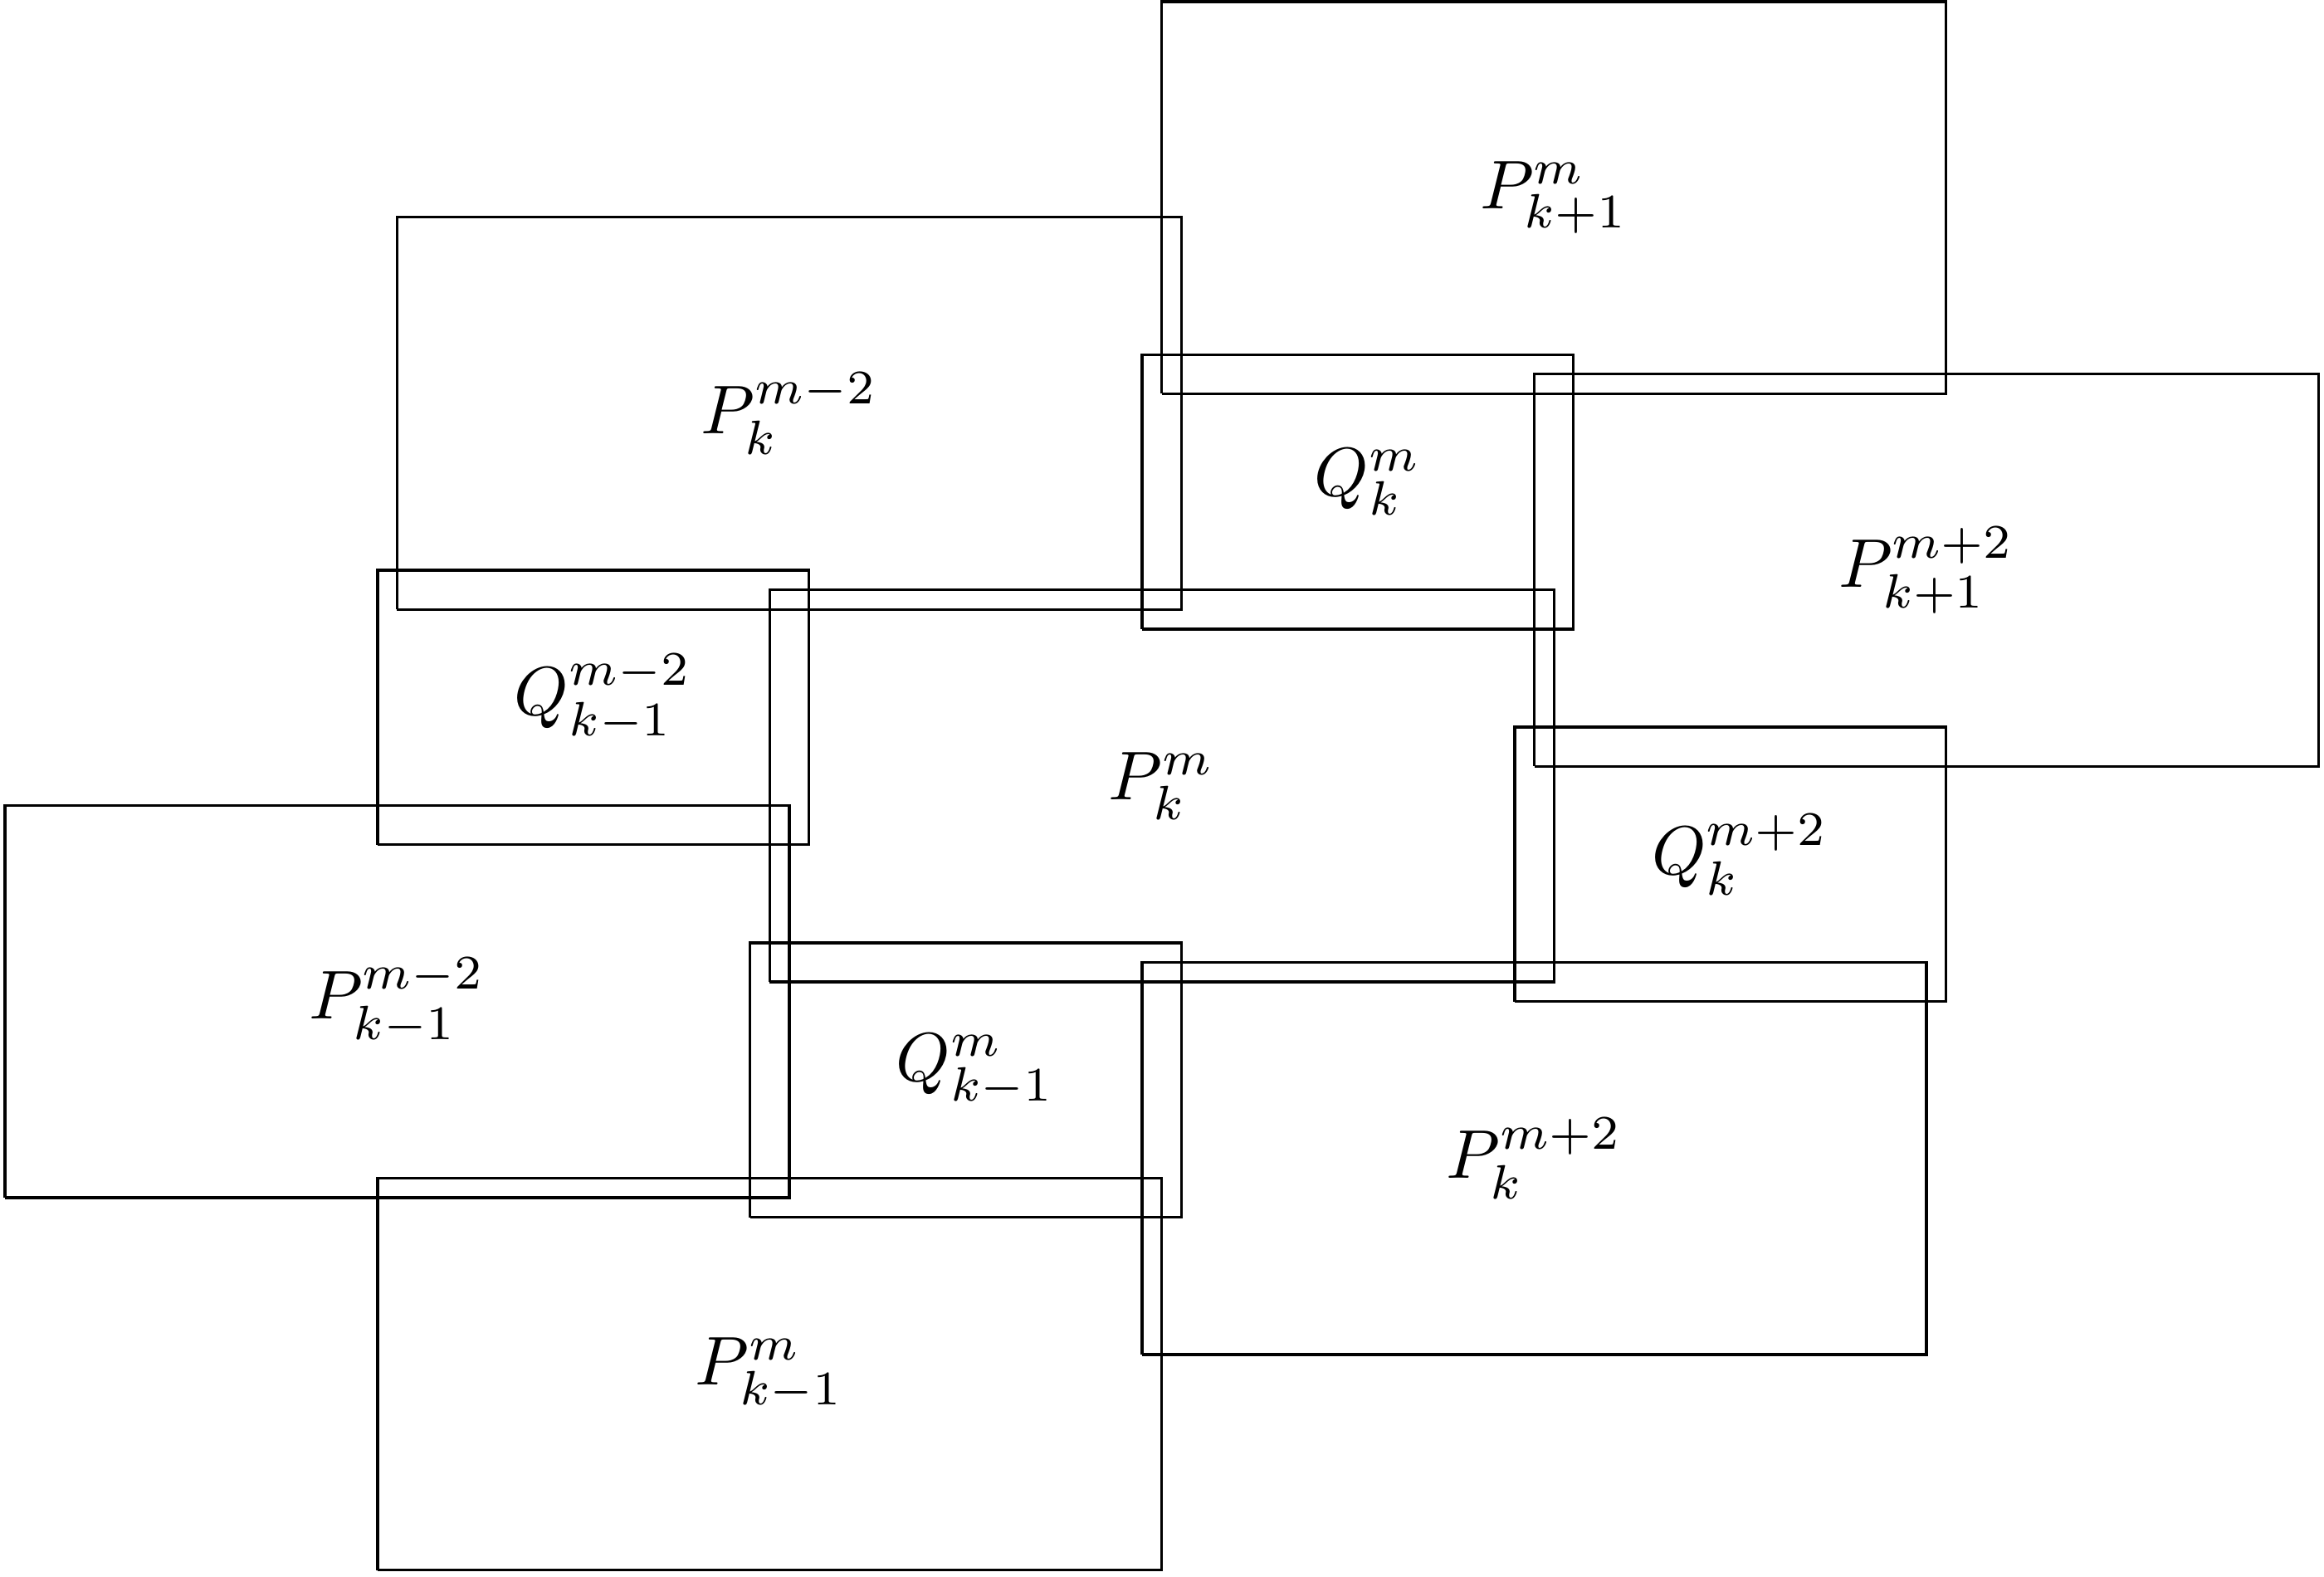
\includegraphics[width=.25 \textwidth]{../Figures/7/7.9a/schema.png}
		\label{fig:add.change.schema.before}
	}
	\subfloat[During]{
		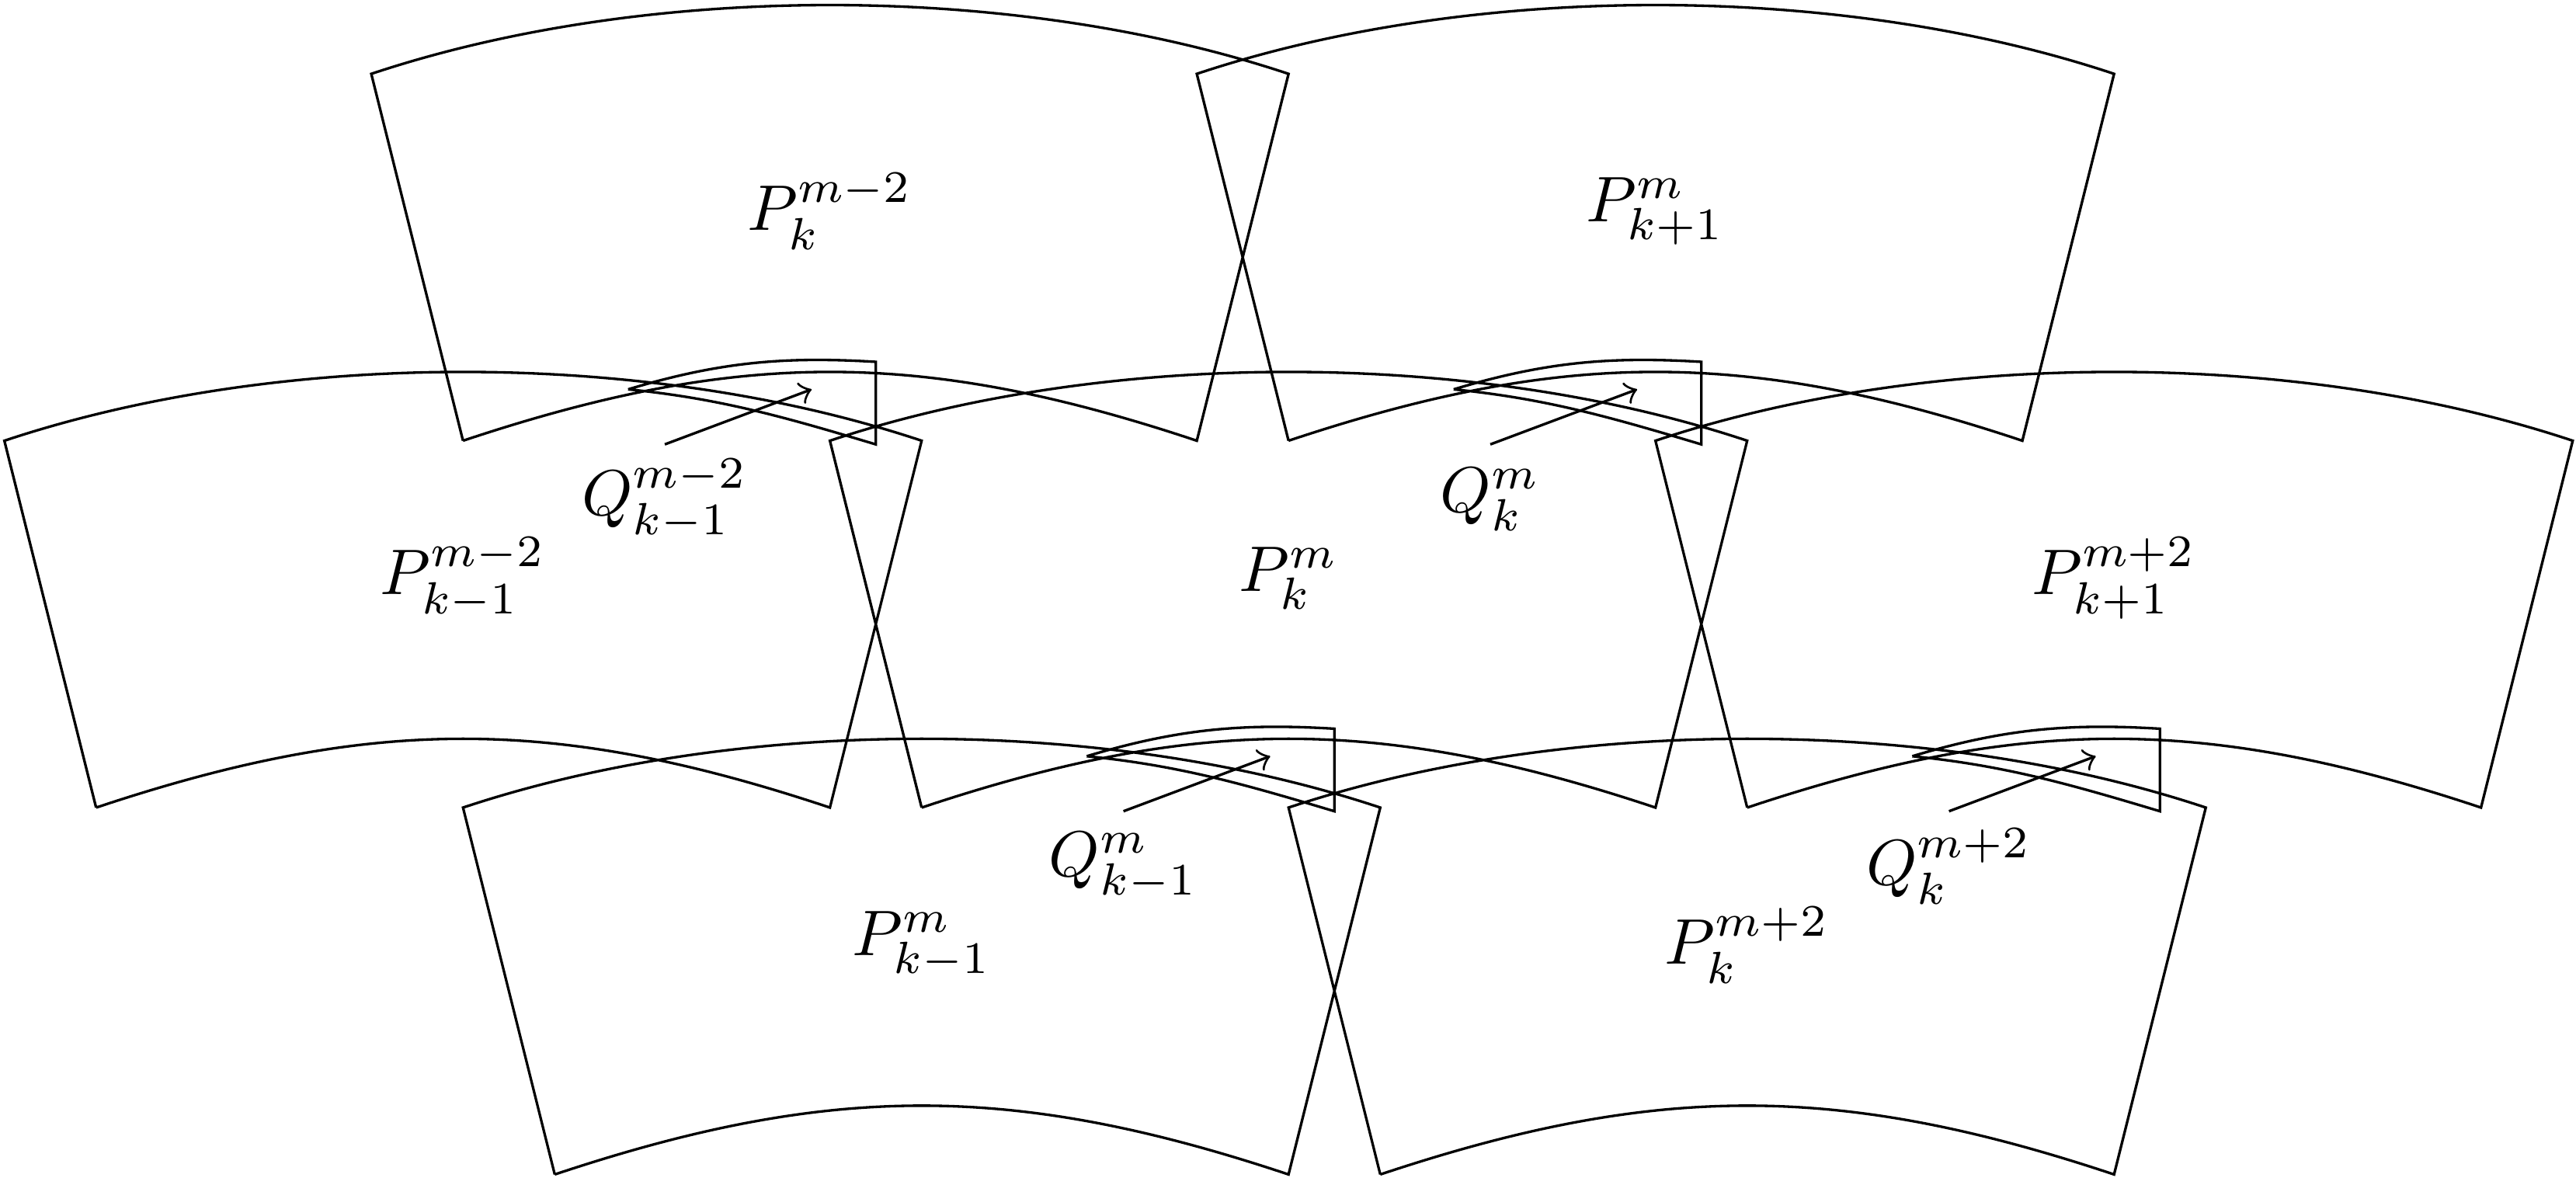
\includegraphics[width=.35 \textwidth]{../Figures/7/7.9b/schema.png}
		\label{fig:add.change.schema.during}
	}
	\subfloat[After]{
		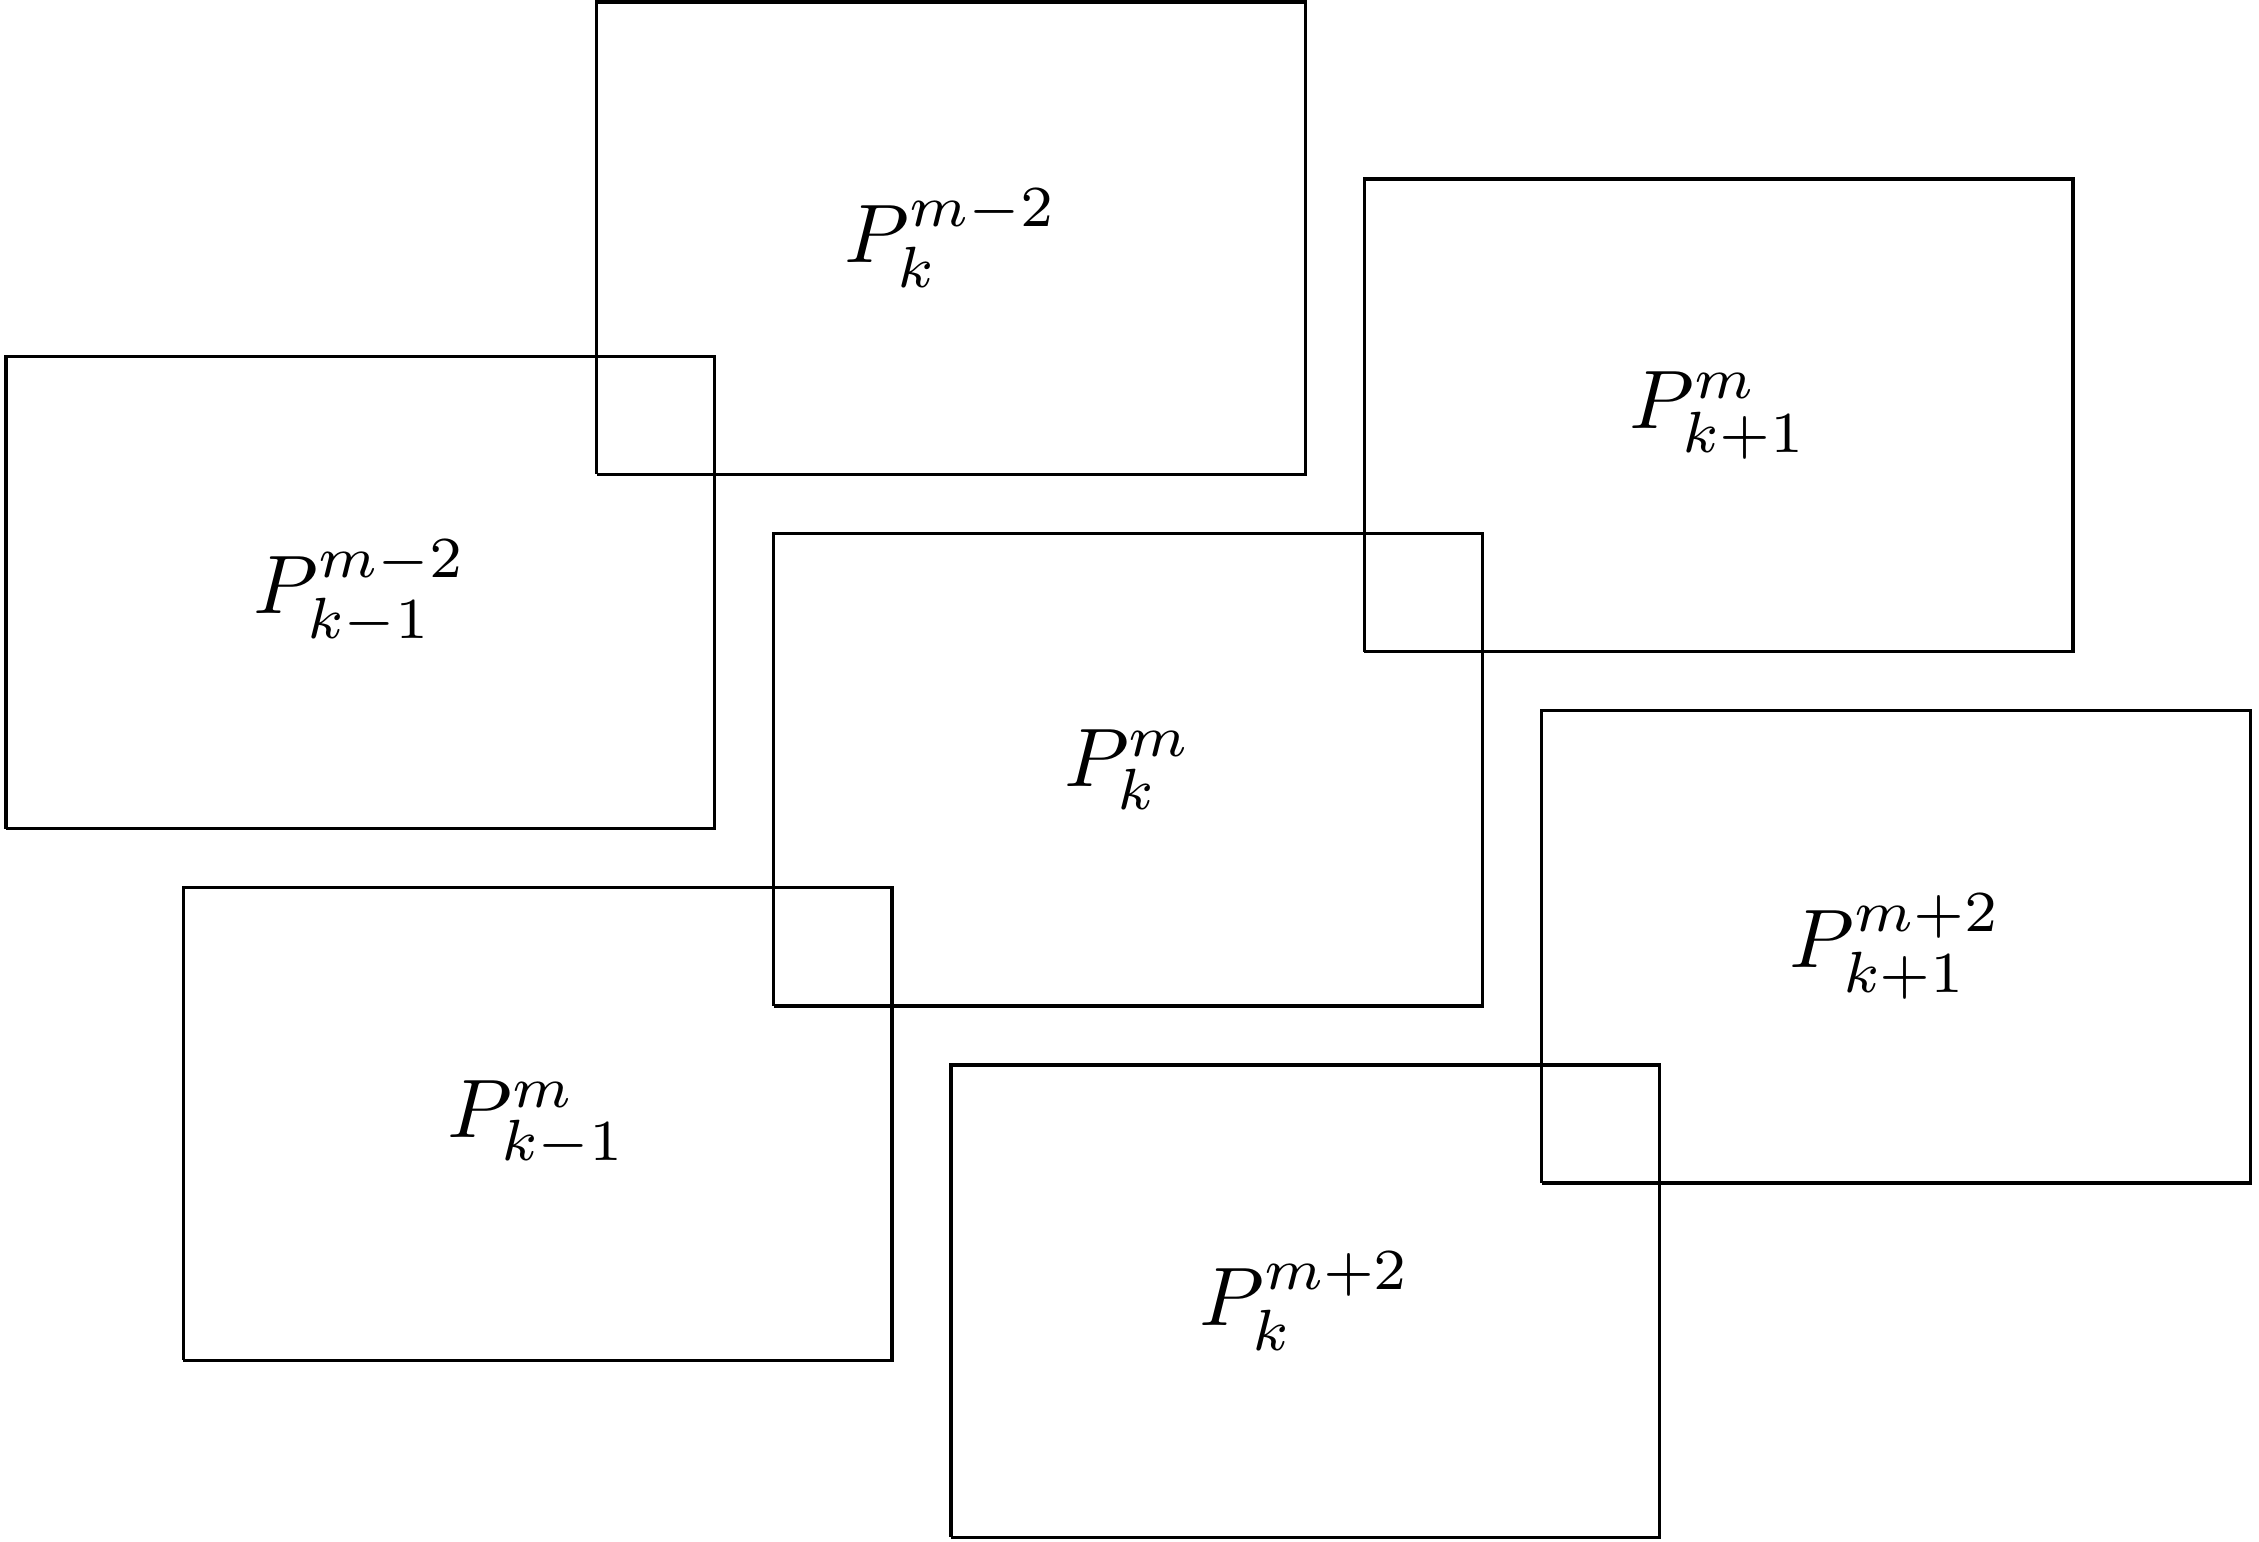
\includegraphics[width=.25 \textwidth]{../Figures/7/7.9c/schema.png}
		\label{fig:add.change.schema.after}
	}
	\caption[Schematics of parameter region boundaries during the transformation of the archetypal model]{
		Schematics of parameter region boundaries during the transformation of the archetypal model.
		(a) shows the parameter regions before the changes start occurring.
		(b) shows the parameter regions with all changes in progress.
		Here we assume that the vertical neighboring ``type A'' parameter regions stop overlapping with a codimension-2 point that moves up.
		And (c) shows the parameter regions after all changes are complete.
	}
	\label{fig:add.change.schema}
\end{figure}

\Cref{fig:add.change.schema} shows schematics of how the boundaries of the ``type A'' and ``type B'' parameter regions change during the transformation into the increasing archetypal model.
Where \Cref{fig:add.change.schema.before} shows the situation before the transformation.
Here, the neighboring ``type A'' parameter regions of different chains overlap and the ``type B'' parameter regions overlap with all neighboring ``type A'' parameter regions.
\Cref{fig:add.change.schema.after} shows the situation after the transformation.
Here the ``type A'' parameter regions of different chains do not overlap, but the ``type A'' parameter regions inside the chains overlap with each other.
And the ``type B'' parameter regions disappeared.

\begin{figure}
	\centering
	\subfloat[Straight]{
		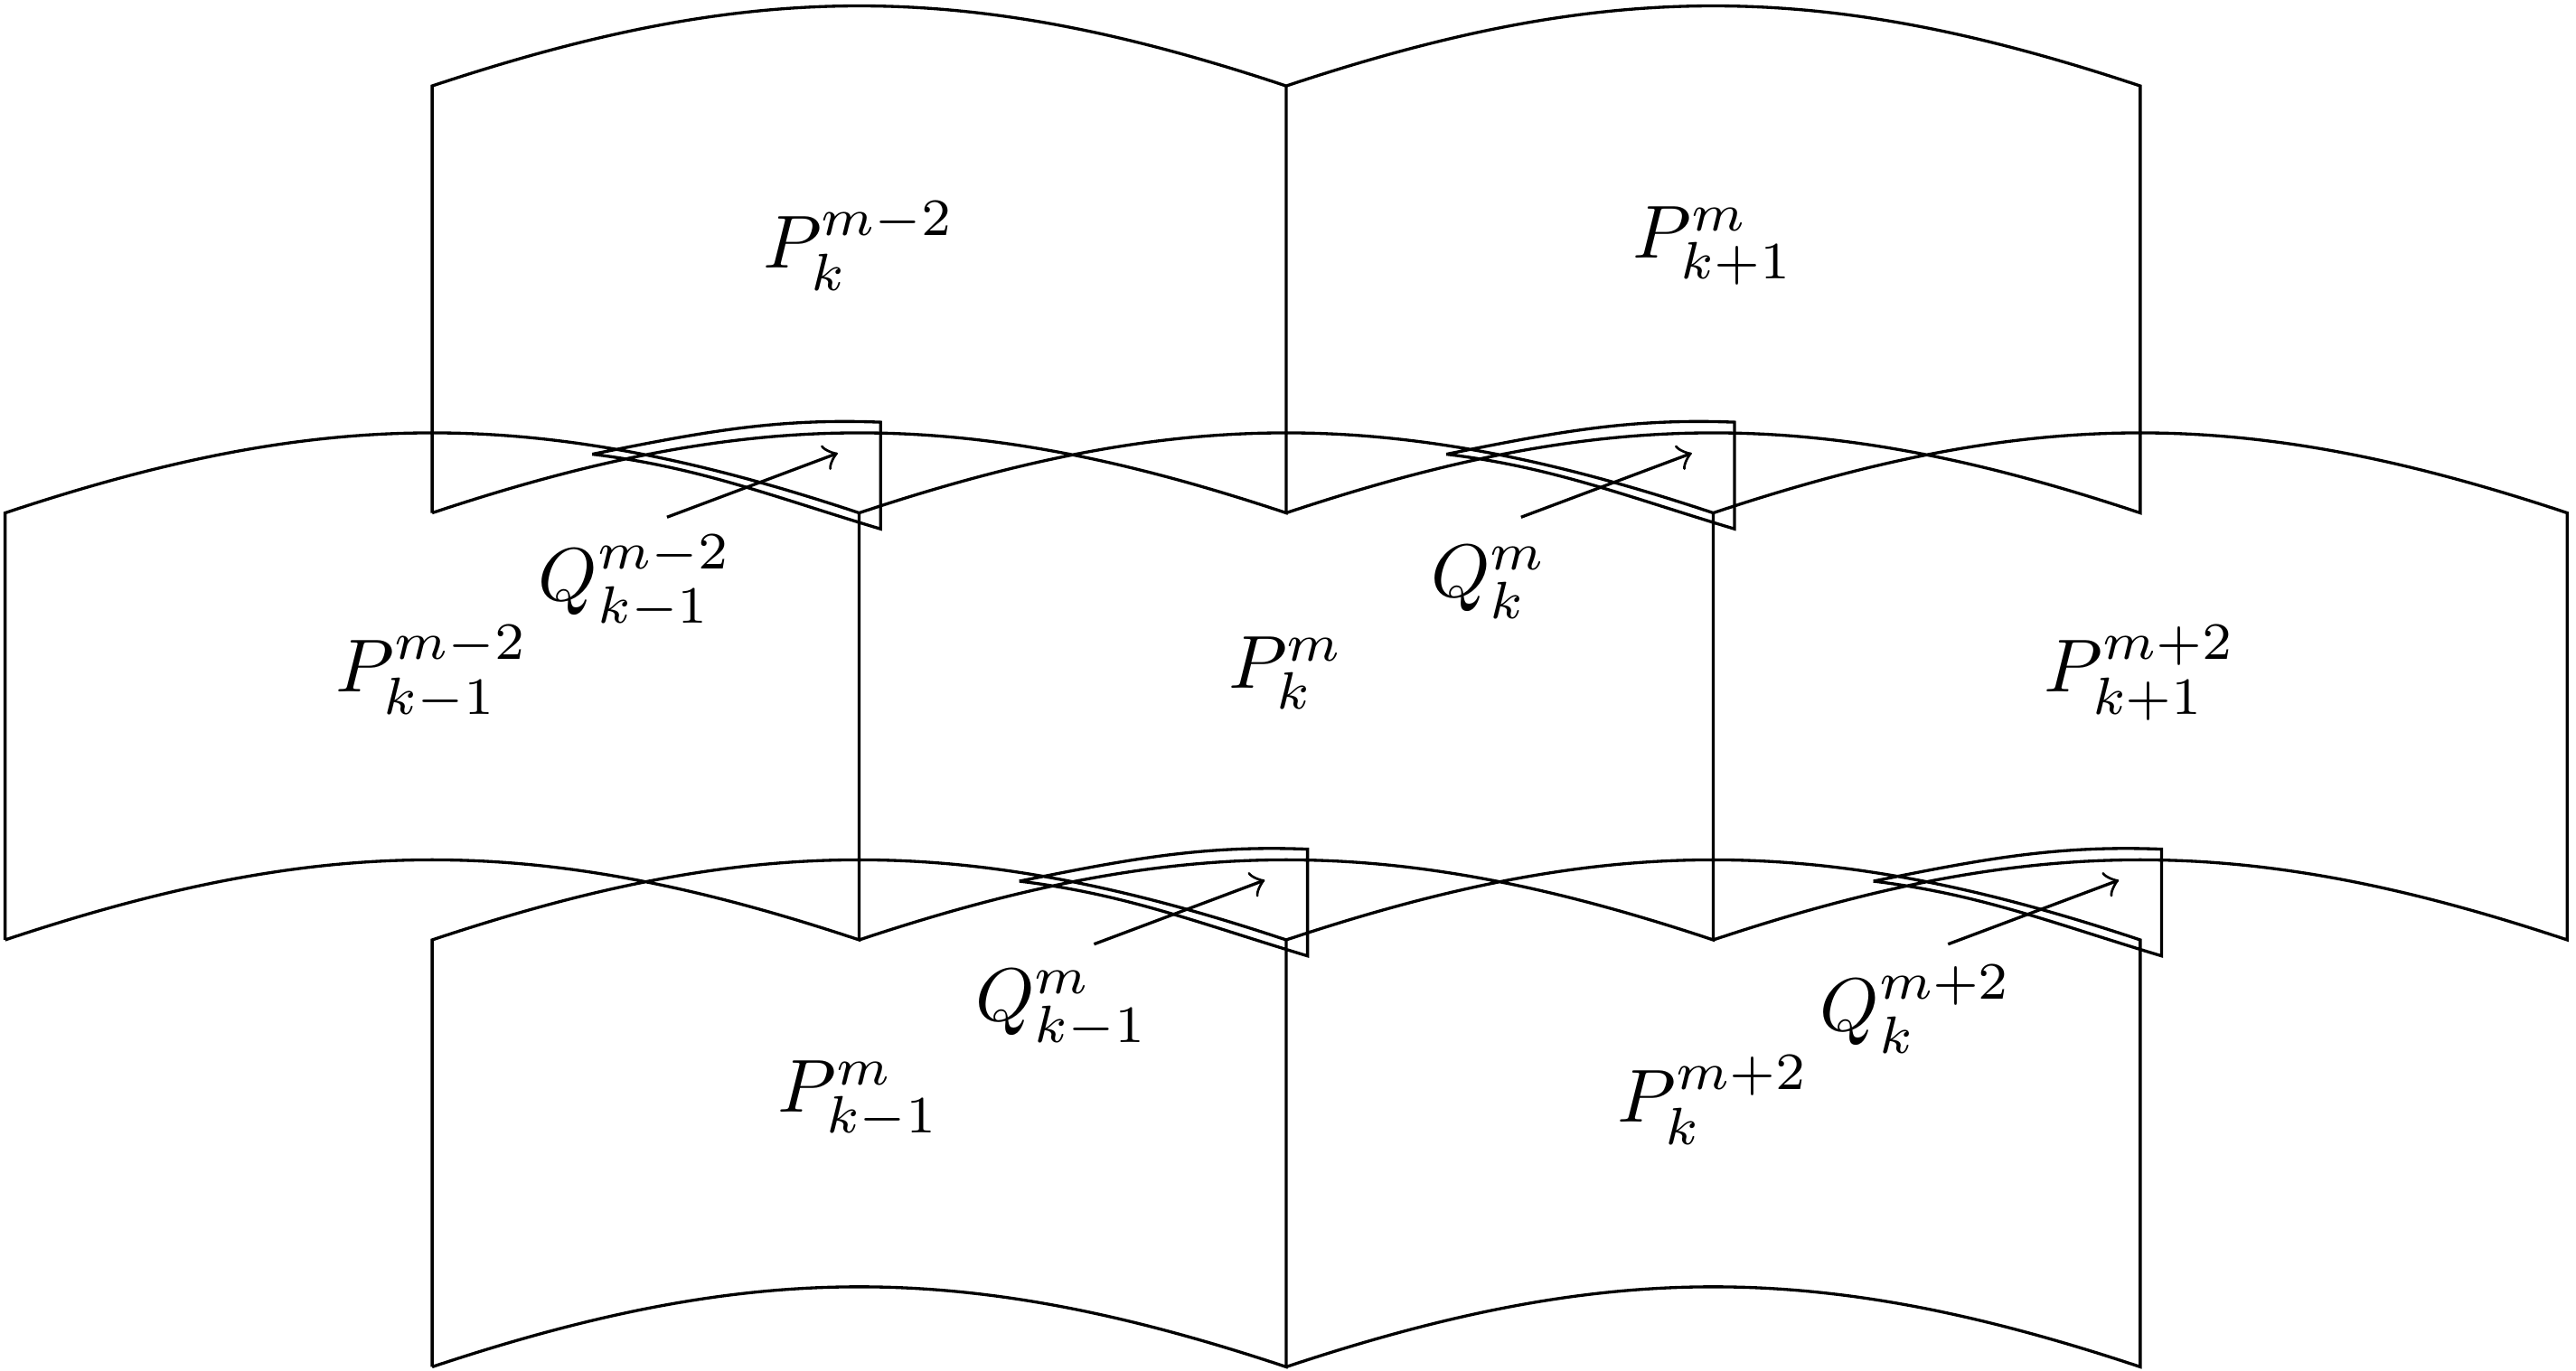
\includegraphics[width=.35 \textwidth]{../Figures/7/7.10a/schema.png}
		\label{fig:add.change.schema.during.straight}
	}
	\subfloat[Inverted]{
		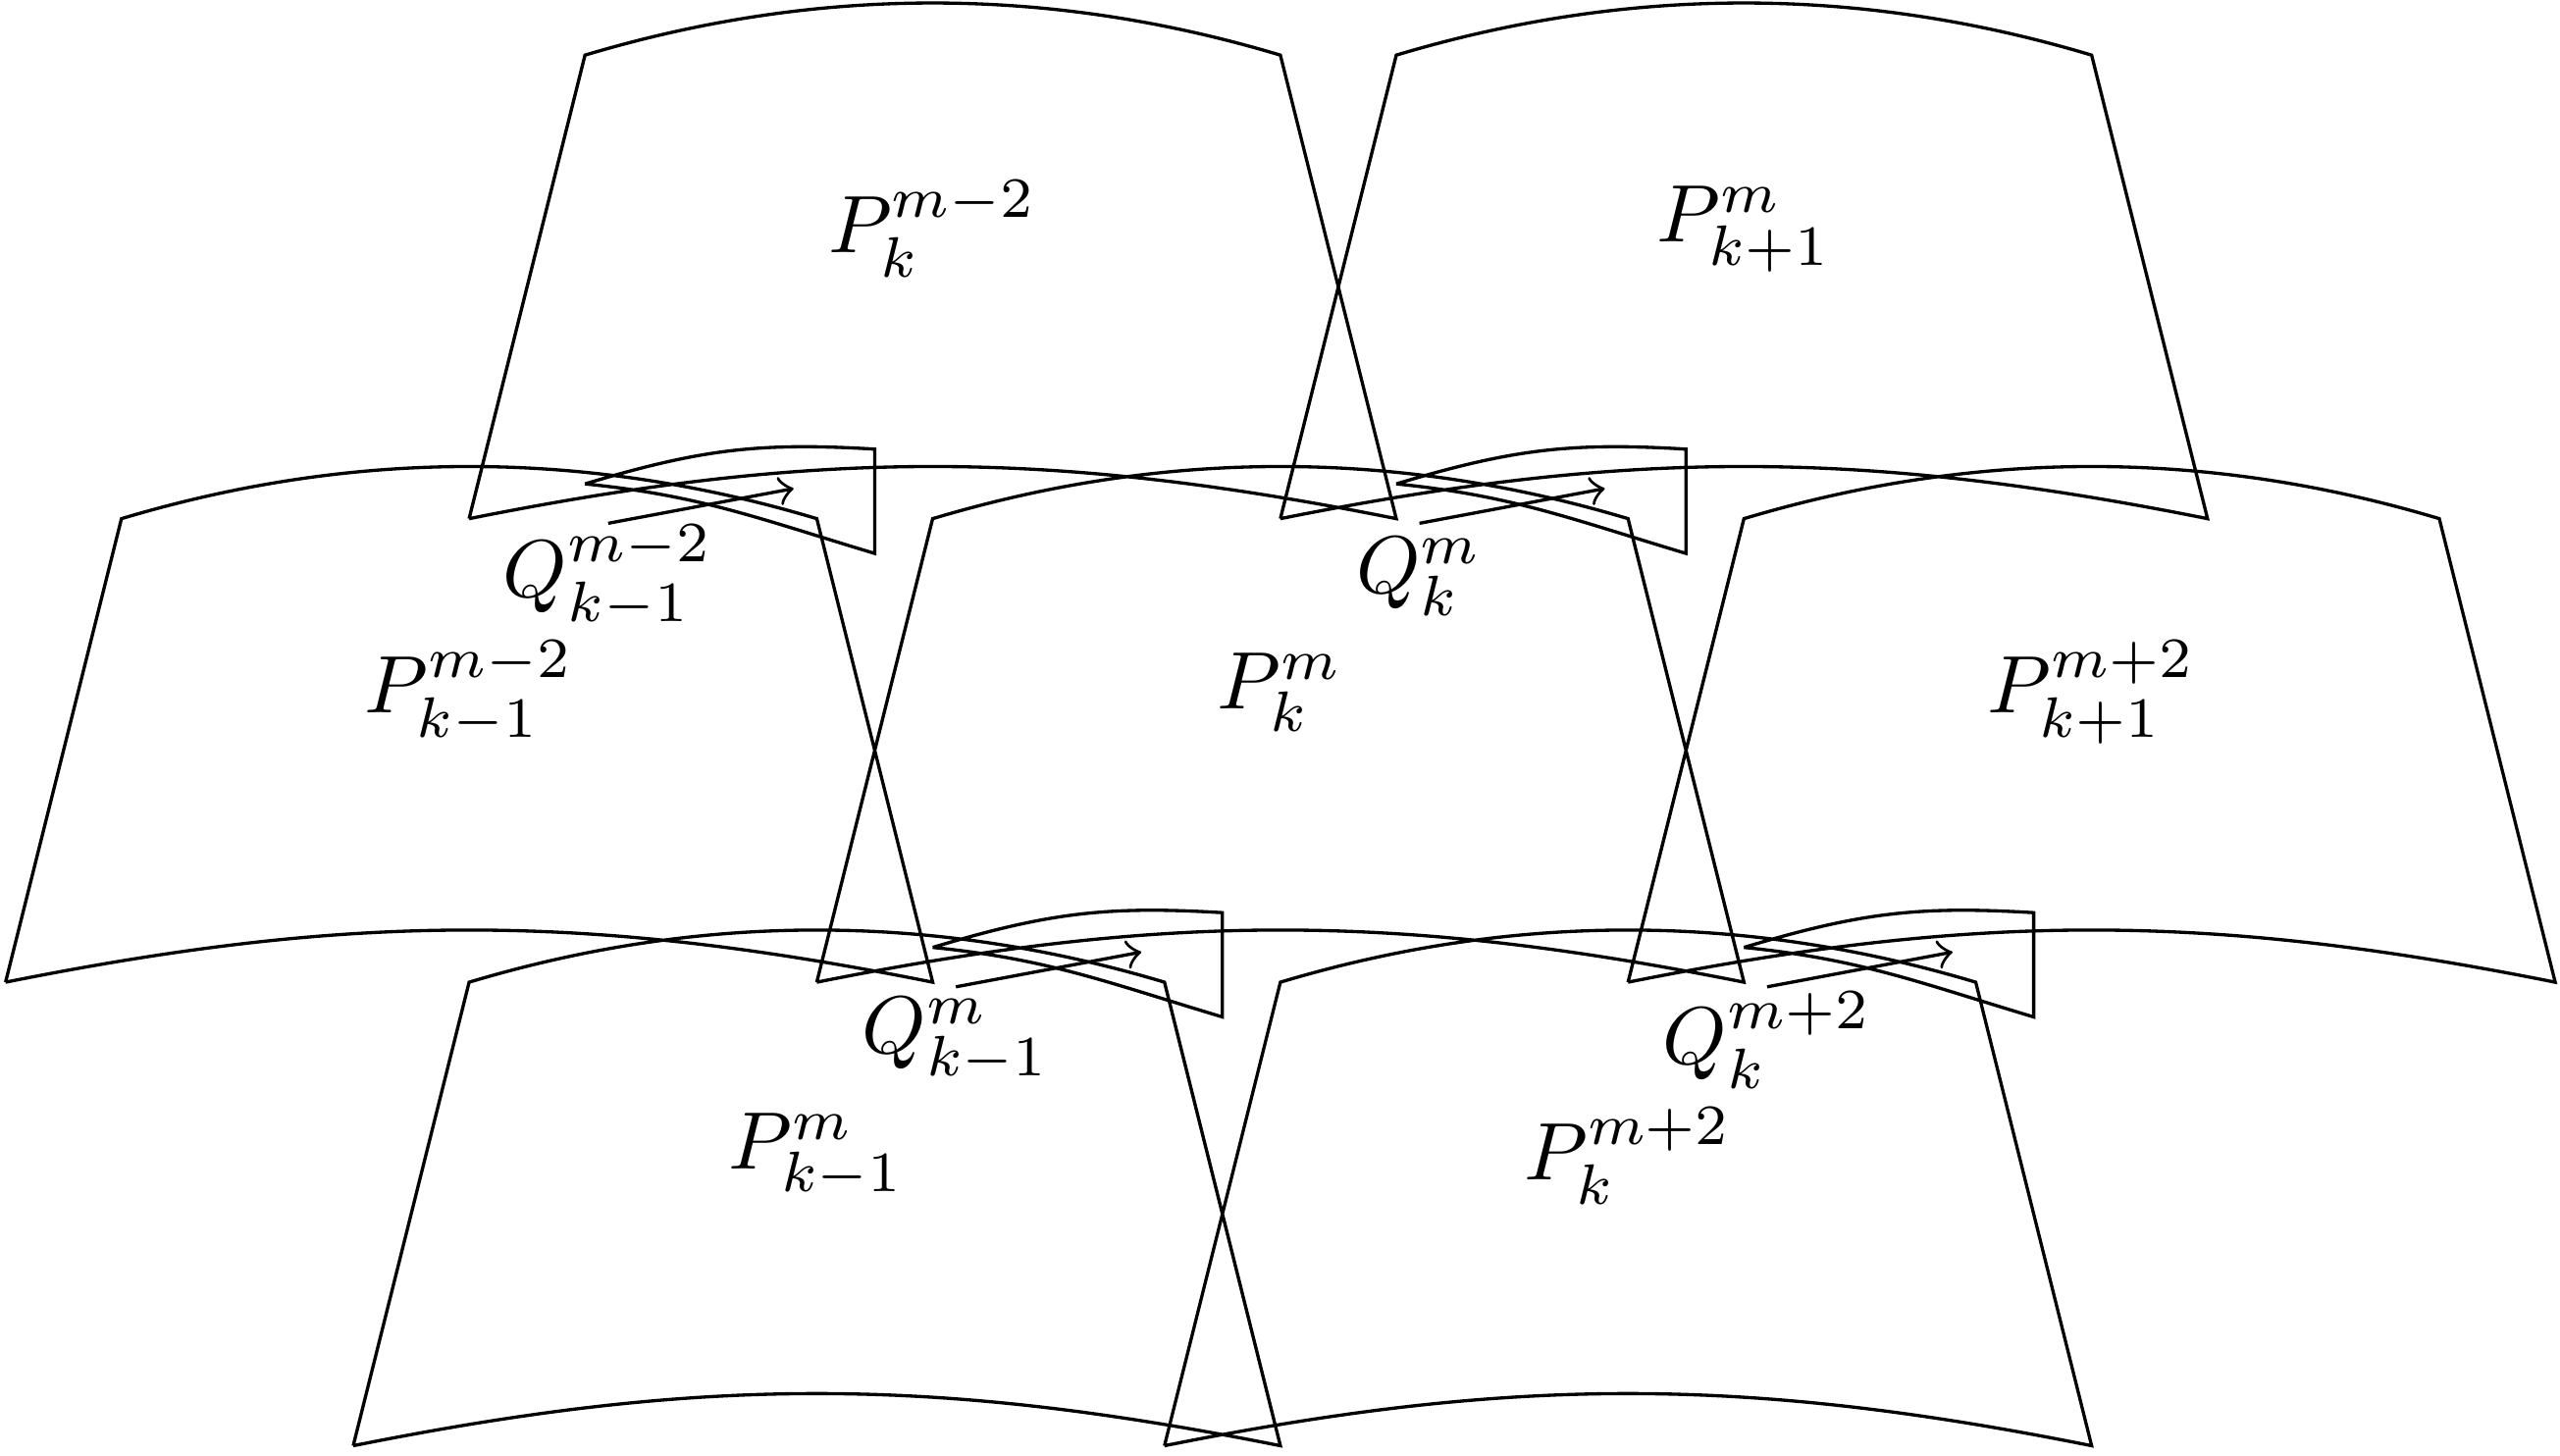
\includegraphics[width=.35 \textwidth]{../Figures/7/7.10b/schema.png}
		\label{fig:add.change.schema.during.inverted}
	}
	\caption[Alternative schematics of parameter region boundaries during the transformation of the archetypal model]{
		Schematics of parameter region boundaries during the transformation of the archetypal model showing alternative cases for the borders between horizontal neighboring ``type A'' parameter regions.
		(a) shows the scenario, if the overlapping period disappears at once with the boundaries aligning perfectly.
		And (b) shows the scenario, if the overlapping period disappears with a codimension-2 point that moves down.
	}
	\label{fig:add.change.schema.during.alt}
\end{figure}

Between those two situations, the boundaries might look like in \Cref{fig:add.change.schema.during}.
Here, the ``type A'' parameter regions of the same chain start overlapping with each other on the left side of their shared boundaries.
The ``type A'' parameter regions of different chains that neighbor vertically stop overlapping on the left side of their shared boundaries.
And finally the ``type A'' parameter regions of different chains that neighbor horizontally stop overlapping on the lower side of their shared boundaries.
We don't have any numerical observations supporting the last case.
The ``type A'' parameter regions of different chains that neighbor horizontally might separate differently.
\Cref{fig:add.change.schema.during.alt} shows alternative schematics for this stage of the transformation.
In \Cref{fig:add.change.schema.during.straight}, the vertical boundaries of horizontally neighboring ``type A'' parameter regions are perfectly parallel.
All the other boundaries stay the same.
And in \Cref{fig:add.change.schema.during.inverted}, the horizontally neighboring ``type A'' parameter regions start separating at the upper side of their shared boundaries.
In this case the codimension-2 point moves down during the transformation.

\subsubsection{Observations}

The local minima on branches $f_\A$ and $f_\C$ seem to be important for the ``type B'' parameter regions.
That means, parameter regions with coexisting asymmetrical cycles with the \textbf{same} period.
At the same time, these minima seem to prevent period-adding structures.
In the following, we will provide a proof that ``type B'' parameter regions are impossible with only increasing branches.

\begin{theorem}[No ``Type B'' Parameter Regions with only Increasing Branches]
	The ``type B'' parameter regions are not possible in the increasing archetypal model.
	The minima on the branches $f_\A$ and $f_\C$ are essential for the bifurcation structure.
\end{theorem}

\begin{proof} \phantom{x} \\
	Let's assume that all branches of the archetypal model $f_\A, f_\B, f_\C,$ and $f_\D$ are increasing.
	And let $\sigma_1$ and $\sigma_2$ be ``type B'' twin cycles.
	The following conditions are true for such cycles.
	\begin{subequations}
		\begin{align}
			|\sigma_1|_\A - 1 & = |\sigma_2|_\A \label{equ:add.change.conseq.sigmaA} \\
			|\sigma_1|_\B + 1 & = |\sigma_2|_\B \label{equ:add.change.conseq.sigmaB} \\
			|\sigma_1|_\C + 1 & = |\sigma_2|_\C \label{equ:add.change.conseq.sigmaC} \\
			|\sigma_1|_\D - 1 & = |\sigma_2|_\D \label{equ:add.change.conseq.sigmaD}
		\end{align}
	\end{subequations}

	For \Cref{equ:add.change.conseq.sigmaA} to hold, the first point of $\sigma_1$ on the branch $f_\A$ needs to be left of first point of $\sigma_2$ on this branch, because the branch is increasing.
	At the same time must its last point on this branch be right of the last point of $\sigma_2$ on this branch.
	This way, $\sigma_1$ has exactly one more point on the branch $f_\A$ as required by \Cref{equ:add.change.conseq.sigmaA}.

	The order of the first points on the next branch, $f_\B$, is the same as for the last points on the branch $f_\A$.
	So the first point of $\sigma_2$ on this branch is left of the first point of $\sigma_1$ on this branch.
	For \Cref{equ:add.change.conseq.sigmaB} to hold, its last point on this branch must be right of the last point of $\sigma_1$ on this branch per the same logic as before.

	The order of the first points on the next branch, $f_\C$, is the same as for the last points on the branch $f_\B$.
	So the first point of $\sigma_1$ on this branch is left of the first point of $\sigma_2$ on this branch.
	This is a contradiction, since the first point of $\sigma_1$ on branch $f_\A$ is also left of the first point of $\sigma_2$ on that branch.
	This violates the symmetry.
	Also, \Cref{equ:add.change.conseq.sigmaC} can't be fulfilled if the first point of $\sigma_1$ is left of the first point of $\sigma_2$ on the branch $f_\C$, since this branch is increasing as well.
	\hfill $\blacksquare$
\end{proof}
